\chapter{The Agent}

\vspace{1em}
\hfill
\begin{minipage}[c]{0.55\textwidth}
\raggedleft
\small\itshape
Reinforcement learning is learning what to do, how to map situations to actions, so as to maximize a numerical reward signal.\\[0.5em]
\upshape\footnotesize Richard Sutton and Andrew Barto, \textit{Reinforcement Learning: An Introduction} (1998)
\end{minipage}%
\hspace{0.5em}
\begin{minipage}[c]{0.12\textwidth}
% \includegraphics[width=\textwidth]{figures/ch05_agent.png}
\end{minipage}
\vspace{1.5em}

\noindent Most of the AI you have heard about falls into one of three categories. The categories overlap (today's systems often combine them), but reading them out as a list is the simplest orientation tool the field has.

\begin{itemize}
\item \textbf{Supervised learning.} You give the system many examples of inputs paired with desired outputs. The system learns the input-to-output mapping. Image classifiers learn from labeled images. Translators learn from sentence pairs. The next-token predictors inside large language models learn from sequences where the ``target'' for each position is just the next token in the text.

\item \textbf{Unsupervised learning.} You give the system data without labels. The system learns the structure of the data on its own. Clustering, dimensionality reduction, compression, density estimation. There is no target to match; the system tries to describe what it sees.

\item \textbf{Reinforcement learning.} The system is an \emph{agent} that acts in an environment. The environment responds with observations and a reward signal. The agent's job is to learn a strategy that maximizes total reward over time.
\end{itemize}

Figure~\ref{fig:trichotomy} places the book's spine on these categories.

\begin{figure}[h]
\centering
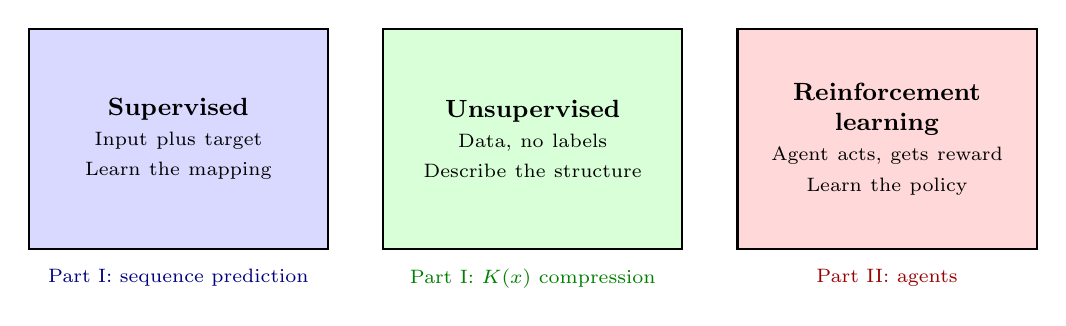
\begin{tikzpicture}[scale=0.9, every node/.style={align=center, font=\small}]
  \node[draw, thick, fill=blue!15, minimum width=3.8cm, minimum height=2.8cm, text width=3.4cm] (sup) at (0, 0) {\textbf{Supervised}\\[0.3em]\scriptsize Input plus target\\\scriptsize Learn the mapping};
  \node[draw, thick, fill=green!15, minimum width=3.8cm, minimum height=2.8cm, text width=3.4cm] (uns) at (5, 0) {\textbf{Unsupervised}\\[0.3em]\scriptsize Data, no labels\\\scriptsize Describe the structure};
  \node[draw, thick, fill=red!15, minimum width=3.8cm, minimum height=2.8cm, text width=3.4cm] (rl) at (10, 0) {\textbf{Reinforcement learning}\\[0.3em]\scriptsize Agent acts, gets reward\\\scriptsize Learn the policy};

  \node[font=\scriptsize, anchor=north, blue!50!black] at (0, -1.7) {Part I: sequence prediction};
  \node[font=\scriptsize, anchor=north, green!50!black] at (5, -1.7) {Part I: $K(x)$ compression};
  \node[font=\scriptsize, anchor=north, red!60!black] at (10, -1.7) {Part II: agents};
\end{tikzpicture}
\caption{The three main categories of machine learning, with the book's spine placed on them. Part I addressed supervised learning in its optimal-limit form (sequence prediction: Solomonoff induction predicts the next observation from a prefix, where the target is just the next bit) and unsupervised learning in its optimal-limit form (Kolmogorov complexity $K(x)$ is the description length of $x$ in its shortest compressed form). Part II addresses the third category: reinforcement learning, with agents acting in environments.}
\label{fig:trichotomy}
\end{figure}

Part I has been about supervised and unsupervised learning in their optimal-limit forms. Solomonoff induction predicts the next observation given a prefix, weighting hypotheses by description length. That is sequence prediction, which is supervised learning where the ``label'' for each position is the next observation. Kolmogorov complexity is the description length of a string in its shortest compressed form. That is unsupervised compression in its idealized limit.

Part II is the move to reinforcement learning. The agent acts; the world responds; the agent updates and acts again. The mathematics inherits Part I (the agent still forms beliefs, and the beliefs are still Bayesian) but adds one ingredient: \emph{stakes}. The agent has values; the actions have consequences with values attached.

This chapter introduces the agent. The rest of Part II builds out what optimal agency looks like.

\section*{What an agent is}

An agent is something with three pieces.

\begin{itemize}
\item \textbf{Perception.} A way of observing the environment. For a robot, sensors. For a language-model agent, text input. For an animal, sight and sound and touch.

\item \textbf{Action.} A way of acting on the environment. Motors, output tokens, words, movements.

\item \textbf{Belief and decision.} Internal machinery that takes perceptions in and produces actions out. Beliefs about the environment, plus rules for deciding what to do.
\end{itemize}

A thermostat is the simplest worked example. Its perception is a thermometer reading. Its action is a switch that turns the heater on or off. Its belief and decision collapse to a single comparison: if the reading is below the target, turn the heater on; if above, turn it off. The thermostat fits in a few lines of logic, and it keeps a house warm. Most other agents are thermostats with more elaborate sensors, more elaborate actions, and more elaborate decision rules.

The agent and the environment form a loop. The agent observes; updates its beliefs; chooses an action; the action affects the environment; the environment generates new observations; the loop continues. Figure~\ref{fig:agent-loop} shows the structure.

\begin{figure}[h]
\centering
\begin{tikzpicture}[
  scale=1.0,
  every node/.style={align=center, font=\small},
  >=Stealth
]
  \node[draw, thick, fill=blue!20, rectangle, rounded corners, minimum width=2.8cm, minimum height=2cm] (agent) at (0, 0) {\textbf{Agent}\\[0.3em]\scriptsize beliefs\\\scriptsize policy};
  \node[draw, thick, fill=gray!15, rectangle, rounded corners, minimum width=2.8cm, minimum height=2cm] (env) at (7, 0) {\textbf{Environment}};

  \draw[->, thick, blue] ([yshift=0.4cm]agent.east) -- node[above, font=\scriptsize, blue!50!black, midway] {action $a$} ([yshift=0.4cm]env.west);
  \draw[->, thick, red] ([yshift=-0.4cm]env.west) -- node[below, font=\scriptsize, red!50!black, midway] {observation $o$, reward $r$} ([yshift=-0.4cm]agent.east);
\end{tikzpicture}
\caption{The agent-environment loop. The agent takes an action; the environment responds with an observation and (in the reinforcement learning case) a reward. The agent updates its beliefs about the environment and chooses the next action. The cycle continues. Everything in Part II lives inside this loop.}
\label{fig:agent-loop}
\end{figure}

The simplest agent is reactive: it observes the environment and picks an action based on a fixed policy. The interesting agents have memory (state from prior steps), planning (consideration of future consequences), and learning (updating policy over time based on outcomes).

Throughout this chapter, \emph{agent} means any system that follows the perception-action loop with internal state. The mathematics applies whether the agent is a thermostat, a chess program, an animal, or an AI system.

\section*{What the agent wants}

An agent is not defined by its perception and action alone. It is also defined by what it wants.

The agent's preferences are encoded by a \emph{utility function}, written $u$. The function maps outcomes to real numbers. Higher numbers mean better outcomes from the agent's view; lower numbers mean worse. Concretely: $u(o) = 5$ means the agent values outcome $o$ at five units; $u(o') = 3$ means it values outcome $o'$ at three. Only the ordering matters in many cases; the units are conventional.

The utility function is the agent's value system. The thermostat's is implicit in what we already described: highest at the target temperature, lower elsewhere. A chess program's might be $+1$ for winning, $0$ for drawing, $-1$ for losing. A human's is much more complex; the function is implicit in behavior rather than written down.

For now, treat $u$ as given. We will return in Chapter 9 to the question of where utility functions come from, why specifying them is harder than it looks, and what happens when the specified utility differs from what the agent (or its designer) actually wants. That is the alignment problem in miniature. For now: $u$ is given.

\section*{Decision under uncertainty}

The agent rarely knows for certain what will happen if it takes a particular action. Most actions have multiple possible outcomes, depending on how the environment responds.

So the agent reasons about expected outcomes, weighted by its beliefs about the environment.

The \emph{expected utility} of an action $a$, given the agent's belief $b$ about the environment, is

$$EU(a) = \sum_{o} b(o \mid a) \cdot u(o).$$

The sum is over possible outcomes $o$. The belief $b(o \mid a)$ is the probability of outcome $o$ if the agent takes action $a$. The utility $u(o)$ is how much the agent values that outcome. Figure~\ref{fig:expected-utility} shows the picture.

\begin{figure}[h]
\centering
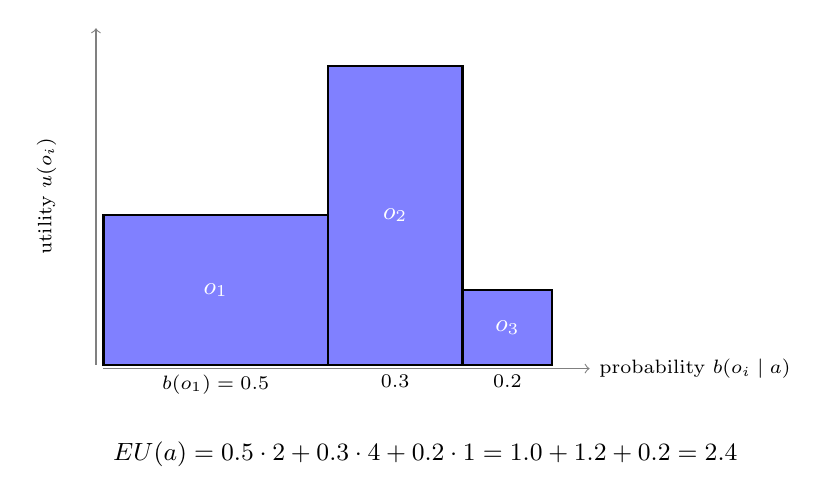
\begin{tikzpicture}[scale=0.95]
  \fill[blue!50] (0, 0) rectangle (3, 2);
  \draw[thick] (0, 0) rectangle (3, 2);
  \node[font=\small, white] at (1.5, 1) {$o_1$};
  \node[font=\scriptsize, anchor=north] at (1.5, 0) {$b(o_1)=0.5$};

  \fill[blue!50] (3, 0) rectangle (4.8, 4);
  \draw[thick] (3, 0) rectangle (4.8, 4);
  \node[font=\small, white] at (3.9, 2) {$o_2$};
  \node[font=\scriptsize, anchor=north] at (3.9, 0) {$0.3$};

  \fill[blue!50] (4.8, 0) rectangle (6, 1);
  \draw[thick] (4.8, 0) rectangle (6, 1);
  \node[font=\small, white] at (5.4, 0.5) {$o_3$};
  \node[font=\scriptsize, anchor=north] at (5.4, 0) {$0.2$};

  \draw[->, gray] (-0.1, 0) -- (-0.1, 4.5);
  \node[font=\scriptsize, rotate=90, anchor=south] at (-0.5, 2.25) {utility $u(o_i)$};
  \draw[->, gray] (0, -0.05) -- (6.5, -0.05);
  \node[font=\scriptsize, anchor=west] at (6.5, -0.05) {probability $b(o_i \mid a)$};

  \node[font=\small, anchor=west] at (0, -1.2) {$EU(a) = 0.5 \cdot 2 + 0.3 \cdot 4 + 0.2 \cdot 1 = 1.0 + 1.2 + 0.2 = 2.4$};
\end{tikzpicture}
\caption{Expected utility as a weighted sum. Each possible outcome $o_i$ of an action $a$ has a probability $b(o_i \mid a)$ (width of the bar) and a utility $u(o_i)$ (height of the bar). The area of each bar is the outcome's contribution to expected utility. The total area is the expected utility of the action. The agent picks the action whose total area is largest.}
\label{fig:expected-utility}
\end{figure}

The decision rule: \textbf{pick the action that maximizes expected utility.}

The agent considers each available action, computes its expected utility under current beliefs, and picks the one whose expected utility is highest.

\subsection*{A worked example: the umbrella}

You are deciding whether to take an umbrella to work. Two actions: take it, or leave it. Outcomes depend on whether it rains. Suppose your utilities are:

\begin{itemize}
\item Dry without an umbrella (it did not rain, you did not bring one): $u = +2$.
\item Dry with an umbrella (annoying to carry, but dry either way): $u = -1$.
\item Wet (no umbrella, it rained): $u = -5$.
\end{itemize}

Suppose the forecast gives $P(\text{rain}) = 0.3$.

Expected utility of taking the umbrella:

$$EU(\text{take}) = 0.3 \cdot (-1) + 0.7 \cdot (-1) = -1.$$

(You carry it either way; the weather does not matter for this action.)

Expected utility of leaving it:

$$EU(\text{leave}) = 0.3 \cdot (-5) + 0.7 \cdot 2 = -1.5 + 1.4 = -0.1.$$

$-0.1$ beats $-1$. Leave the umbrella.

Now suppose the forecast updates: $P(\text{rain}) = 0.7$.

$EU(\text{take}) = -1$ (unchanged).
$EU(\text{leave}) = 0.7 \cdot (-5) + 0.3 \cdot 2 = -2.9$.

Now $-1$ beats $-2.9$. Take the umbrella.

The belief changed; the utility function did not. The decision flipped. That is what decision under uncertainty means: the right action depends on what you think the world will do.

\section*{Why expected utility}

You might ask why this rule. Why not the best worst case (the minimax pessimist)? Why not the best best case (the maximax optimist)? Why not something nonlinear in the probabilities, like prospect theory's risk-weighted version?

In 1944, John von Neumann and Oskar Morgenstern showed that under modest consistency requirements, any rational agent acts \emph{as if} it is maximizing the expected value of some utility function.

The requirements are short:

\begin{itemize}
\item \textbf{Completeness.} For any two outcomes, the agent has a preference: either it prefers one, or the other, or it is indifferent.
\item \textbf{Transitivity.} If the agent prefers $a$ to $b$, and $b$ to $c$, then it prefers $a$ to $c$.
\item \textbf{Continuity.} If the agent prefers $a$ to $b$ to $c$, then there is some probability mixture of $a$ and $c$ that the agent is indifferent to receiving in place of $b$.
\item \textbf{Independence.} Preferences between two gambles do not depend on irrelevant common parts: if you prefer $a$ to $b$, you also prefer ``$a$ or $c$ each with probability one-half'' to ``$b$ or $c$ each with probability one-half.''
\end{itemize}

Under these axioms, the agent's preferences over gambles can be represented by a utility function such that the agent prefers gamble $g_1$ to gamble $g_2$ if and only if the expected utility of $g_1$ exceeds the expected utility of $g_2$.

\subsection*{What goes wrong when the axioms fail}

To see why the axioms matter, consider what happens when they are violated. Suppose your preferences fail transitivity: you prefer $A$ to $B$, $B$ to $C$, and yet $C$ to $A$.

I can drain your money indefinitely. Start with you holding $A$. I offer to trade $A$ for $C$ plus a small fee. You accept (you prefer $C$). Now you hold $C$. I offer to trade $C$ for $B$ plus another fee. You accept (you prefer $B$). Now you hold $B$. I offer to trade $B$ for $A$ plus another fee. You accept (you prefer $A$). You are back to holding $A$, three fees lighter. The cycle can run as long as you have money.

This is the \emph{money pump} argument. Any agent with intransitive preferences can be drained without limit. Transitivity is not arbitrary; it is the requirement that prevents you from being a perpetual mark.

Similar arguments cover the other axioms. Violating independence makes you vulnerable to constructed gambles (the Allais and Ellsberg paradoxes are well-known cases where humans systematically violate independence and the consequences can be exploited). Violating continuity gives an exploit at the boundary between alternatives. Each axiom corresponds to closing a specific exploit.

The full vNM result is: the only way to rank gambles consistently, without being exploitable, is to maximize expected utility for some utility function.

\subsection*{Other criteria, in disguise}

Some criteria that look unlike expected utility maximization turn out to be expected utility maximization with a different utility function. Minimizing maximum regret (the gap between what you got and what you could have got with perfect hindsight) is expected utility maximization with utility set to negative regret. Risk-aversion can be expressed by making utility a concave function of dollars. The framework is broader than it might look at first; what changes between criteria is the utility function, not the underlying rule.

This is structurally the same kind of result as Cox's theorem from Chapter 1. Cox showed that consistency forces belief revision to be probabilistic. Von Neumann and Morgenstern show that consistency forces decision under uncertainty to be expected utility maximization. In both cases, a small set of innocent-looking requirements collapses the space of options to a single answer.

It does not say what the utility function \emph{is}. It says: whatever your preferences, if they are consistent, they can be represented this way. Where the preferences come from is, like the prior, a separate question.

\section*{Where this leaves you}

You have an agent. It perceives. It acts. It has beliefs (from Part I, updated by Bayes with a principled prior). It has a utility function over outcomes (the value system, given for now). It decides by computing expected utility for each available action and picking the maximum.

This is the core of decision theory. The rest of Part II builds out its consequences.

\textbf{Chapter 6 (Reinforcement Learning)} takes the static picture and adds time. The agent does not decide once; it decides repeatedly, with future actions depending on observations not yet made. Exploration vs exploitation enters as a structural feature: should the agent take its best current bet, or try something less proven in order to gain information that might lead to a better bet later? Value of information is what answers this question.

\textbf{Chapter 7 (Generalization)} confronts a fact the static picture hides: a real agent meets more situations than it could ever tabulate, so it must generalize from finite experience to the unseen. That means function approximation, inductive bias, and the architectures of modern machine learning.

\textbf{Chapter 8 (AIXI)} synthesizes Part I and Part II. Solomonoff induction for the prediction half. Expected utility maximization for the decision half. Combined: AIXI, the optimal universal agent. Uncomputable, but the right reference point for what intelligence is in the limit.

Then Part III opens. \textbf{Chapter 9 (Reward Modeling)} returns to the utility function. We have been treating $u$ as given. Specifying it is harder than it looks. Goodhart's law is the warning sign; the alignment problem is what follows when the specification fails at scale.

The next chapter takes the first step.
